\section{User Engagement in micro videos}
\label{sec:classifier}
We begin our analysis by devising a novel 
methodology to analyze how the previously defined features impact user engagement in micro videos (\textbf{RQ1}). Our results indicate the importance of social features for highly engaging videos, and that the presence of faces is a strong content-related feature that positively impacts user engagement.
%: We build a machine learning model that predicts  engagement with high accuracy, precision and recall. The  relative feature importances then indicate what aspects of the micro videos matter more to users. By varying the threshold of engagement, we can analyse how different features change for high and low engagement items.  %First, we discuss our experiment setup and then present the model's performance and discuss the implications: that content-related features are collectively more important than social features for engagement, and that presence of faces is the single most important content-related feature.

\subsection{Metrics and methodology}
\label{sec:methodology}
To understand which aspects or features are important for user engagement, we need to: \one\ define a metric for engagement, and \two\ develop a methodology to study how the metric is influenced by different features. 

\noindent\textbf{Defining a metric for user engagement}:  In this paper, we  use \emph{number of loops} of a micro video as a proxy for user engagement towards it\footnote{We obtained similar trends using number of reposts, but only report results with loops. Note that the loop counts of videos are highly correlated with reposts and likes. For example for videos in POP12K, $ corr(Loops,Likes) = 0.80$, $corr(Likes,Reposts) = 0.91$, $corr(Reposts,Loops) = 0.74$.}.
Although user engagement is a broadly used term, and other metrics may well be used to represent user engagement, our choice is in line with previous related social media studies (e.g.~\cite{bakhshi2014faces})  that have used social attention metrics such as likes and comments to study user engagement. Video hosting platforms like Youtube also use the number of views (similar to number of loops on Vine) as a core metric for their user engagement API\footnote{\scriptsize https://developers.google.com/youtube/analytics/v1/dimsmets/mets}. In the rest of the paper, we will use popularity and engagement interchangeably.

\noindent\textbf{Motivating the methodology}: 
 Given a set of features, if we can build a machine learning model that uses the features to predict which content items are highly engaging, the relative importance of the different features in making the prediction can tell us about the relationship between the features and engagement. However, our results will only be as `good' as the model is in predicting loop counts. Since predicting popularity with exact numbers such as loop counts is a hard problem, we turn to a simpler one: We define an arbitrary threshold count for loops, and categorize micro videos as popular or unpopular depending on whether the loop count is over or under the threshold.  We then design a classifier that predicts whether a micro videos is popular or unpopular (alternately, as engaging or not) based on our set of 28 features (Table~\ref{tab:Features_table}) . As discussed next, a simple random forest classifier can be trained to make this prediction with high precision and accuracy. The relative importance of different features then tells us about how the features affects user engagement.

This method has one major limitation: its dependence on the arbitrarily defined loop count threshold. Therefore, we conduct a  sensitivity analysis by training a series of binary classifiers for different loop count thresholds. This also allows us to study shifts in relative importance, as we move up the scale towards more popular and engaging objects, by defining increasingly higher numbers of loop counts as the threshold for categorizing a video as popular (or engaging). 
%
%In this section, we explore user engagement with videos in Vine. Foll
%To understand the processes involved in user engagement with a micro video, we 
% designed various experiments based on supervised learning. Similar to previous work analyzing the impact of images in social media \cite{bakhshi2014faces}, we use social attention metrics as proxy for user engagement. % where in we use machine learning methods, to understand influence of the features used for training, on the engagement classification process. 
%We  use a machine learning framework to understand the relevance of different kinds of features on the overall engagement potential of a micro video and gain some empirical evidence about the impact contribution by each Aesthetic, Audio, Sentiment, Faces and Social feature. 
%%Further to validate our hypothesis about differential impact of the initial seconds on the engagement against the rest of the video, we train two classifiers where one uses the features across the complete video, and other only across the first 2 seconds. Comparing the performances of both, we were able to conclusively propose the validity of our hypothesis.  
%%
%
%\subsection{Defining User Engagement}
%%\mr{Sagar please write why loops and how you vary thresholds - pasting some stuff that you had written somewhere else} \sj{Please check if this looks good}. 
%For this experiment, we  choose \emph{number of loops} as a proxy for user engagement. %This can be drawn from the fact that several scalable 
%This is inline with previous work on user engagement in social media \cite{bakhshi2014faces}. Moreover, video hosting platforms like Youtube, use the number of views as a core metric for their user engagement API \footnote{https://developers.google.com/youtube/analytics/v1/dimsmets/mets}. However, although social attention metrics such as reposts (revines) , likes and loops are intuitively correlated with user engagement, %but this in varying levels of granularity. 
%quantifying the metric value after  which the user is engaged might not be trivial.   \mr{Nishant I think here we should add something about how this setting can help exposing feature importance?}
%A person may watch a video till the end and would be interested in the video enough to loop it again, or he may go ahead and voluntarily like the video and at the highest level of interaction, he may like the video enough to repost it to his own social network. We are interested in designing an experiment that could regress the impact of the features across all these varying levels of engagements. With this in mind, we vary our definition of "Engaging" by progressively increasing the threshold of Loop count after which a video is labelled as engaging.  We vary such threshold starting from median loop count of ALL120K dataset all the way till 1.5 times the median value of POP12K dataset. So in a nutshell, we make our definition of what classifies as engaging more and more selective.
\subsection{Model details}
\label{sec:model-details}
\noindent\textbf{Setup}
%Due to the exhaustive nature of our data, the computational resources in terms of CPU usage and time would be unmanagable, so 
We sample 12,000 videos from our dataset, out of which 6,000 are popular videos from  POP12K, and 6,000 randomly sampled from the ALL120K dataset, thus representing the entire spectrum of engagement levels. In each video, we sample the video track for individual frames at every second, and extract the audio track as well as meta-data related to the video and its author. Using these, we then compute the 28 dimensional vector of all the features in Table \ref{tab:Features_table} and train a random forest classifier to distinguish popular and unpopular videos for different thresholds of popularity. We used the implementation from the \emph{SKLearn} package with $\sqrt{n_{features}}$ split and $500$ estimators, which provided the best trade-off between speed and prediction performance.
 
\noindent\textbf{Performance Results} 
Different classifiers are trained using the above method for different engagement/popularity thresholds, using an 80-20 split for training and validation. Fig \ref{fig:Classifier_performance} shows how these perform as we vary the threshold of ``engagement'' (popularity) from 80 loops (the median for ALL120K) to  $\approx$ 500,000 loops (1.5 times the median of the popular videos i.e., POP12K). At each training iteration with a changed ``engagement'' threshold, we re-balance the dataset by choosing equal number of samples which fall in either classes. We take care that we are training on at-least 20\% of the complete dataset by the end of the process, and stop increasing the threshold beyond that point to avoid over-fitting. The classifiers gave consistently high performance on the validation dataset (see lines labeled 6 sec), never dropping below 90\% for accuracy, and 80\% F-1 score, validating our next results about the importance of different features. 

\subsection{Feature analysis and implications}
The impact of individual features on user engagement is calculated using Gini importance~\cite{louppe2013understanding}, and combined into social-  and content-related (i.e., audio and video-related) features as described before (\S\ref{sec:features}). Fig.~\ref{fig:Feature_importance} shows the trends in  feature importance as a function of engagement threshold used (see lines labeled 6 sec). We observe that at lower thresholds of popularity, social features are much more important than content-related features, but at higher thresholds, content-related features increase in importance to become just as important as social features, suggesting that \emph{content quality is important for user engagement at the top end of engagement}. This facet of users' engagement with Vine might legitimize Twitter's decision to more closely integrate the Vine platform with its social network: since a large part of micro-video popularity can be explained with social factors, a better social network might further foster engagement with this unique form of expression. %However, it is still unclear whether this closer integration would help promoting  less popular videos  by providing an alternate route of exposure, or will  a diffusion mechanism based purely on social factors limit the access to less popular videos? 

We drill down further in Fig.~\ref{fig:Feature_importance_content}, and examine the importance of different kinds of content-related features. For each class of content-related features, we plot the mean of the feature set of the class. We observe that in terms of effective importance of different feature tracks, sentiment is the weakest influencer in the classifier decision process. We conjecture that the relative lack of importance of sentiments may partly be due to the extremely short nature of micro videos, which does not let emotional `story arcs' and plots (e.g., drama) to develop as strongly as in longer videos.
%We do this by finding the mean of a set of feature importances corresponding to a particular set of features. 
%Amongst aesthetic, the Luo Simplicity was the most dominant for 5 classifier train iterations and then colour contrast becomes dominant for the rest of the train iterations. Among the Audio features, short-time energy ,which is a measure of sudden loudness, is dominant for the first 25 train iterations . At the highly selective range , Rhythemical features or Zero crossing rate , which measure the rhythmical content of a waveform , become dominant. 


Further, we observe that the presence of faces in a frame strongly outweighs all other content-related features in predicting popularity. %\ns{document which is the dominant feature of each kind}
We confirm this in Figure~\ref{fig:Face_CDF} by comparing the percentage of faces in popular POP12K videos with the corresponding percentage in ALL120K videos (which contain a large number of unpopular videos as well as a few popular ones).  These results indicate that popular videos tend to have more faces, i.e., ``\emph{faces engage us}''. This is in alignment with similar results on other platforms, which also indicate that faces greatly enhance popularity related metrics such as likes and comments~\cite{bakhshi2014faces}. 


% \begin{figure}[!htb]
% \centering
% 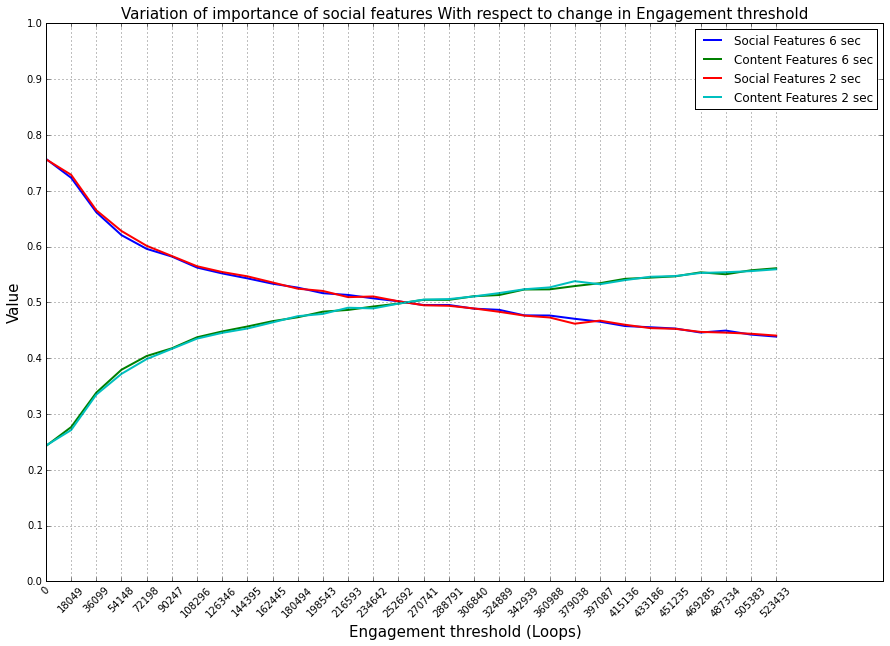
\includegraphics[width=0.5\columnwidth]{plots/socialVsContent6sec2sec}
% \caption{\textsl{ A plot of contribution of social features against all the perceptual features combined. The influence is calculated by training the classifier and looking at the coefficients of the final classifier. The plot shows Social Vs Content feature importance for a classifier trained on the whole 6 Second video and that trained on just the first 2 seconds }}
% \label{fig:Feature_importance}
% \end{figure}

\begin{figure*}[htp]
\centering

\subfloat[ Content Vs Social Features ]{
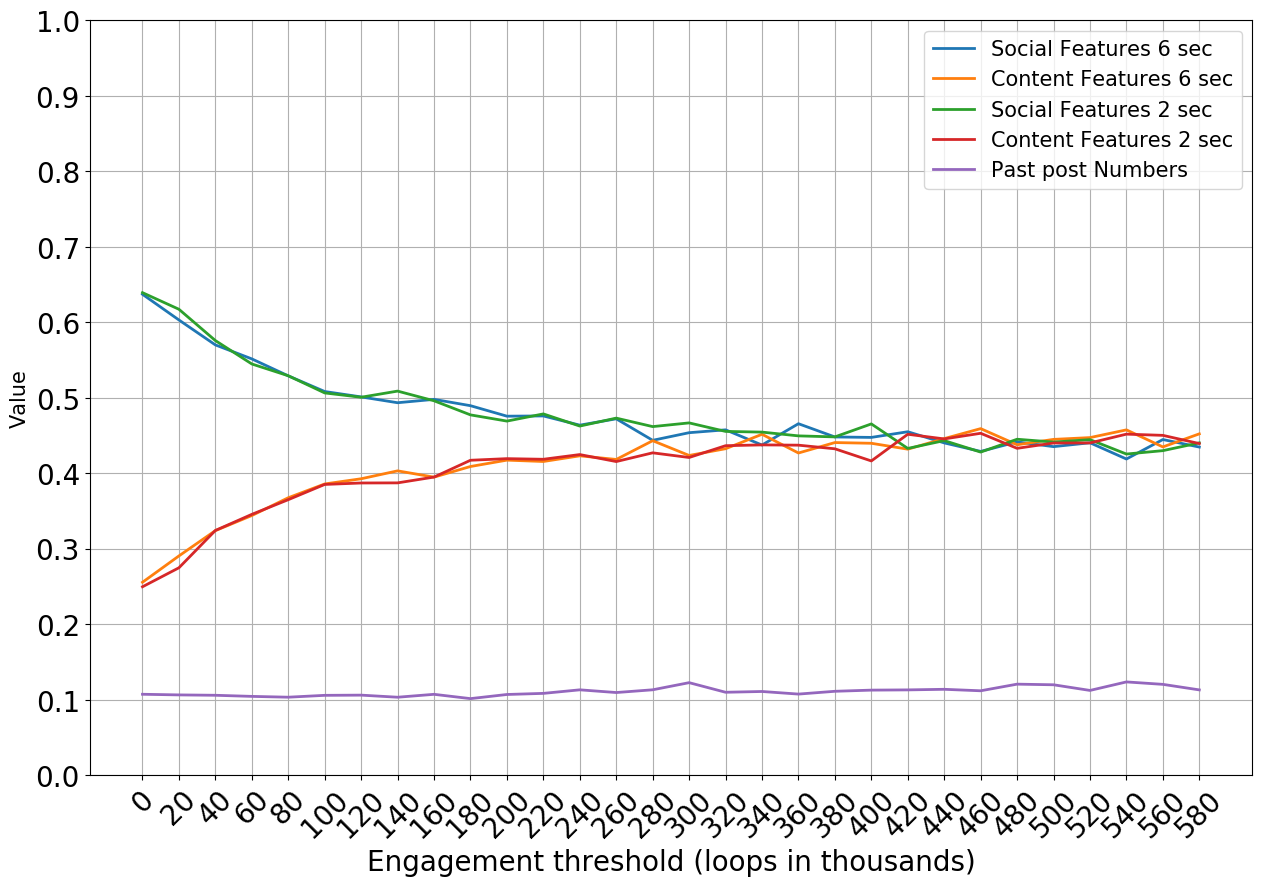
\includegraphics[width=0.5\textwidth, height = 4.5cm ]{plots/engagement}
\label{fig:Feature_importance}
}
\subfloat[ Individual Content Features ]{
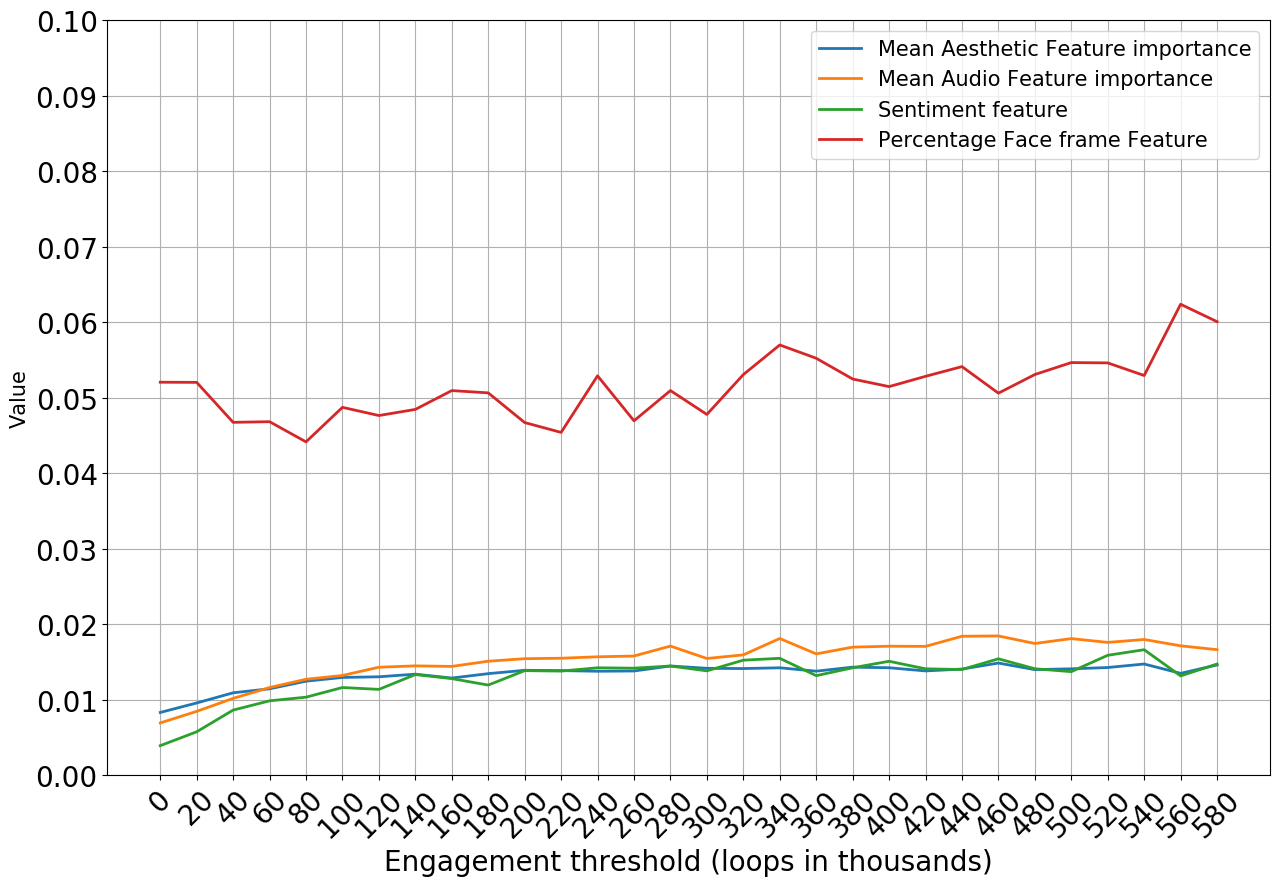
\includegraphics[width=0.5\textwidth, height = 4.5cm]{plots/contentFeatures}
\label{fig:Feature_importance_content}
}

\subfloat[ Classifier Performance ]{
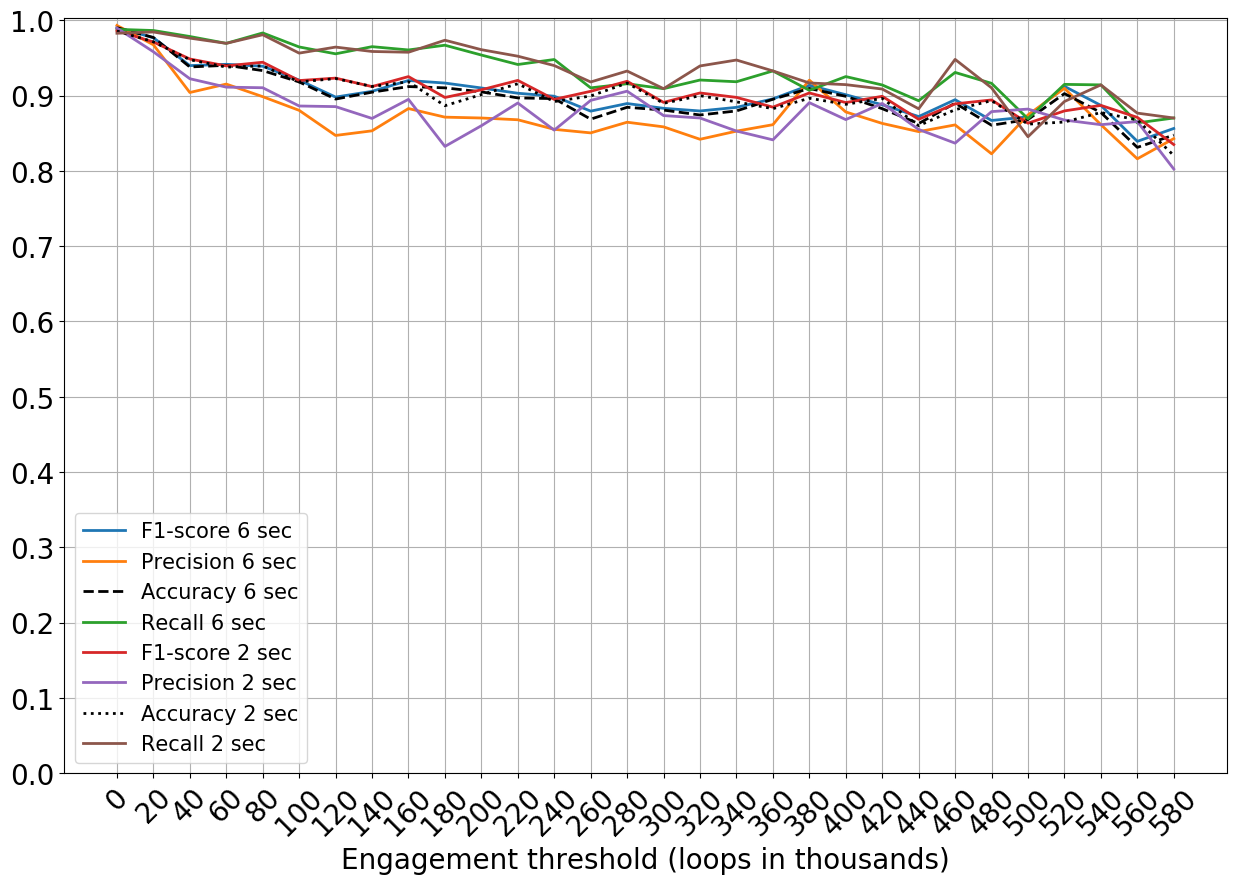
\includegraphics[width=0.5\textwidth, height = 4.5cm]{plots/classifier_accuracy}
\label{fig:Classifier_performance}
}
\caption{ Understanding engagement for different thresholds (min.\ number of loops considered as engaging). Two different classifiers are used, one using quality of the entire micro video (labeled 6 sec), the second measuring quality from only the first two seconds (labeled 2 sec). (a) As threshold becomes higher, content-related factors become as important as social factors (both classifiers). Note that unlike content quality computed from the first 2 seconds (`Content features 2 sec') rather than the entire 6 seconds of the video (`Content features 6 sec'), `social features 6 sec' uses the same feature values as Social Features 2 sec', but the two are plotted separately to show the relative  importance of social features in the 6 second vs 2 second classifier. (b) Amongst content features alone, presence of faces in the video is the single most dominant feature, across all threshold levels (6 second classifier) (c) Both 2 sec and 6 sec classifiers perform similarly across all metrics such as Precision, Recall and F1-score. Performance is high across all engagement thresholds: all metrics are consistently over 0.8 or 0.9.}
\label{fig:classifier}
\end{figure*}




\begin{figure}[!htb]
\centering
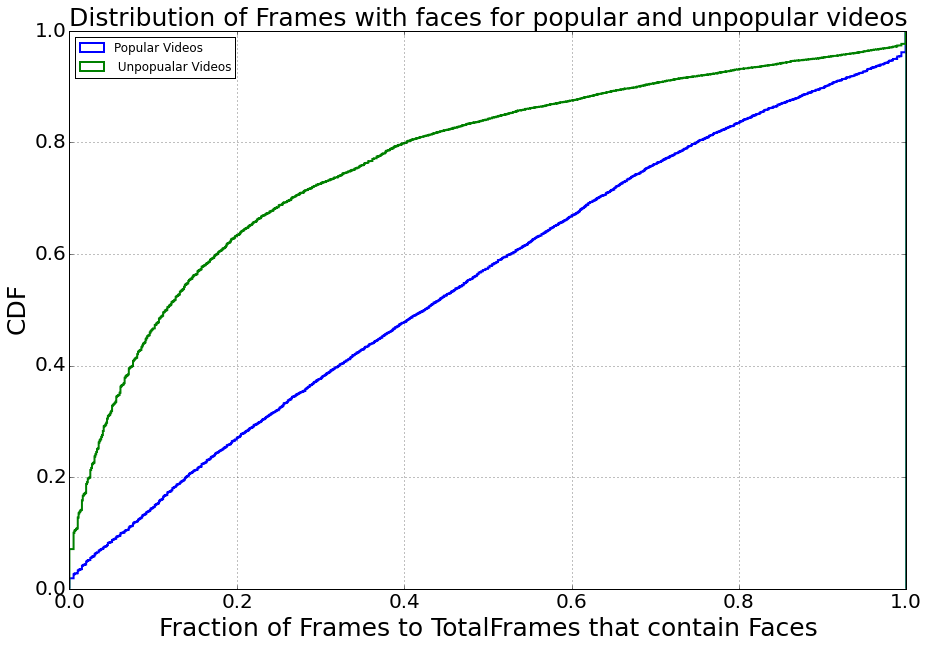
\includegraphics[width=0.6\columnwidth]{plots/FaceCDF}
\caption{\textsl{ CDF for popular and unpopular videos. The CDF signifies the cumulative distribution of percentages of frames containing faces in a vine video. The observation here is popular videos tend to have higher face percentage than unpopular videos}}
\label{fig:Face_CDF}
\end{figure}

%\subsection{Feature Analysis: Faces engage us!}
%To understand   the impact of individual features on user engagement we look at the transition of feature importance as a function of engagement threshold. This is done by using  the Gini importance calculation method \cite{louppe2013understanding}. The importance of  distinct tracks for different levels of engagement is shown in Fig. \ref{fig:Feature_importance_content}.
%\vspace{3pt}\\\textbf{Content Matters more than Social Features, Sometimes.}
%Fig. \ref{fig:Feature_importance} shows the variation of the impact of social features, compared with all the other content related features across all the iterations. It is important to note, that the impact of content related features, becomes more decisive as we make our engagement criteria more selective. 
%\vspace{3pt}\\\textbf{Content Features.}
%To understand relative importance of features amongst the content features themselves , we track the importance of aesthetic , audio , sentiment and face feature sets \ref{fig:Feature_importance_content}.
%Each curve corresponds to the most dominant feature amongs a feature set. The reason we don't consider a cummulative effect of each feature set, is then the impact would be disproportionate due to variable length of each feature vector for each set. So the dominant feature gives an overall idea per feature, per feature set, when it comes to their impact. From the Fig \ref{fig:Feature_importance_content}, we can see a notable impact by the Face percentage feature. The impact weight is as high as 10\% at its highest despite being just a scalar feature. This points towards a relatively profound implication covered in the next part.   %\sj{ I am open to change on this one. The current method makes sure Aesthetic featues don't get unfairly shown the most dominant becasue of the sum of 19 feature  dimensions over just one for face and sentiments}
%\mr{Sagar please comment fig:Feature\_importance\_content and fig:Senti\_distribution, what can you say about those? We should conclude that faces are the most important and to link to the next part}
%%
%%
%%
%\vspace{3pt}\\\textbf{Faces engage us.}
%Following this intuition, we further analyse the role of faces for micro-video engagement.
%%For analysing this feature, we run the viola jones face detector for profile and frontal faces on every frame of the selected videos. Once sampled videos were processed for presence of faces, we analysed their prevalence seperately for the high engagement videos sampeld from the POP12K dataset and the low engagement videos sampled from the ALL120K dataset. 
%
%%\begin{figure}
%%\centering
%%\subfloat[\textit{Distribution of sentiment values for Popular and unpopular videos.}]{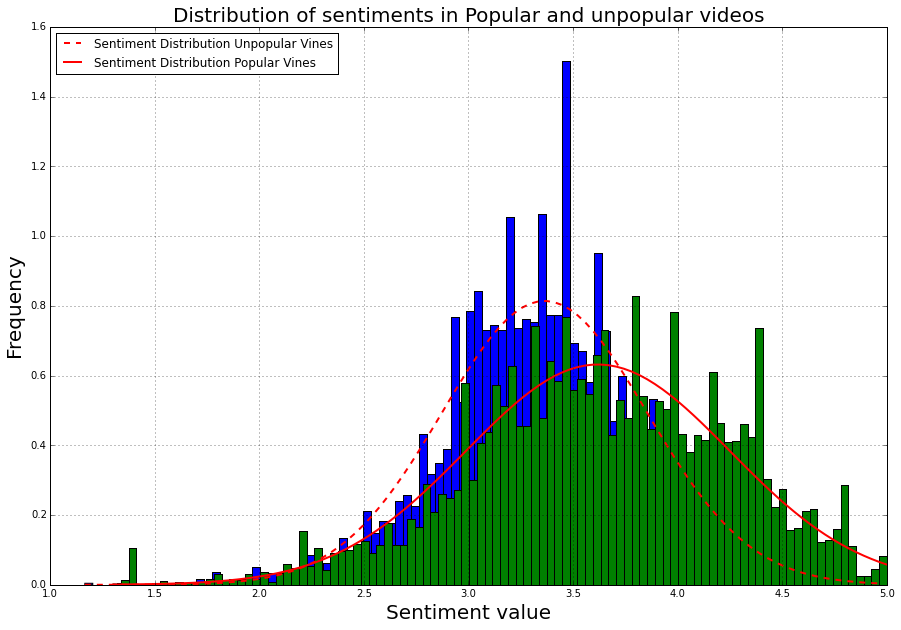
\includegraphics[width=0.5\columnwidth]{plots/DistributionSentiments}}
%%\hfill
%%\subfloat[\textsl{ CDF for popular and unpopular videos. The CDF signifies the cumulative distribution of percentages of face containing frames in a vine video.}]{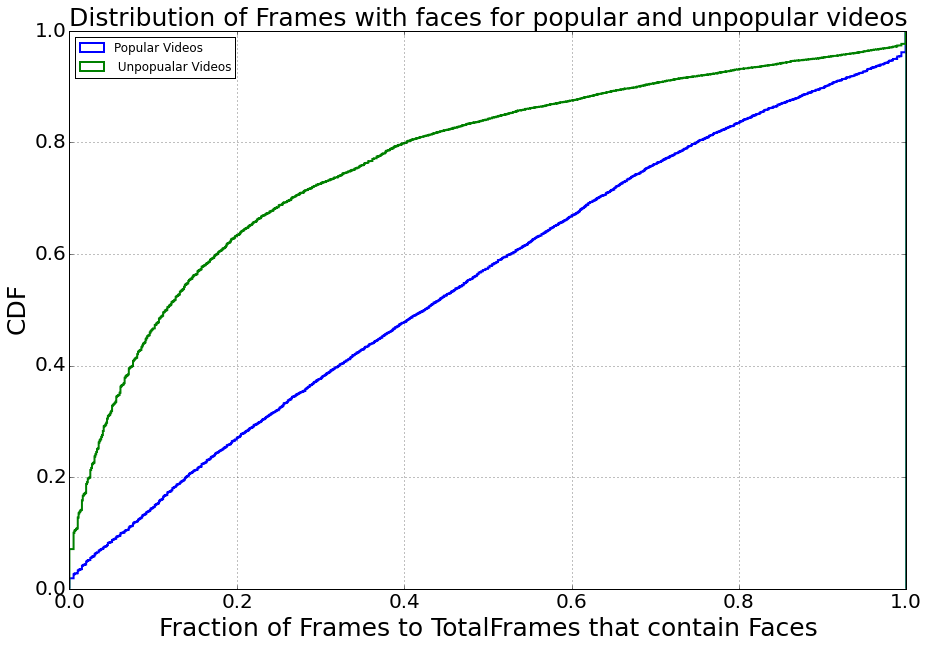
\includegraphics[width=0.5\columnwidth]{plots/FaceCDF}}
%%\hfill\null
%%\end{figure}

%\begin{figure*}[!htbp]
%\centering
%\vspace*{-5mm}
%\subfloat[Distribution of Sentiments , popular and unpopular videos]{
%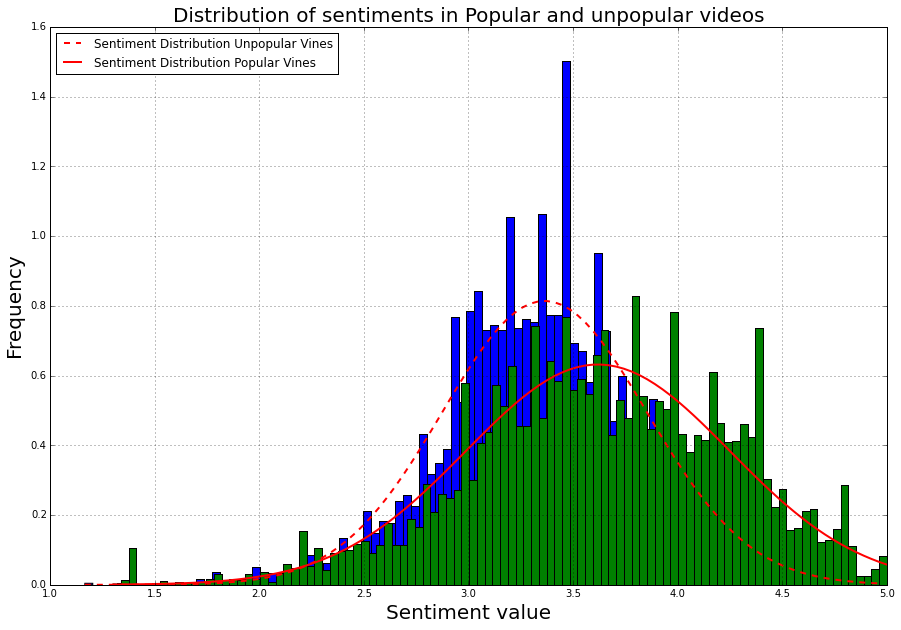
\includegraphics[width=0.45\columnwidth]{plots/DistributionSentiments}
%\label{fig:Senti_distribution}
%}
%\subfloat[CDF for face percentages, popular and unpopular videos]{
%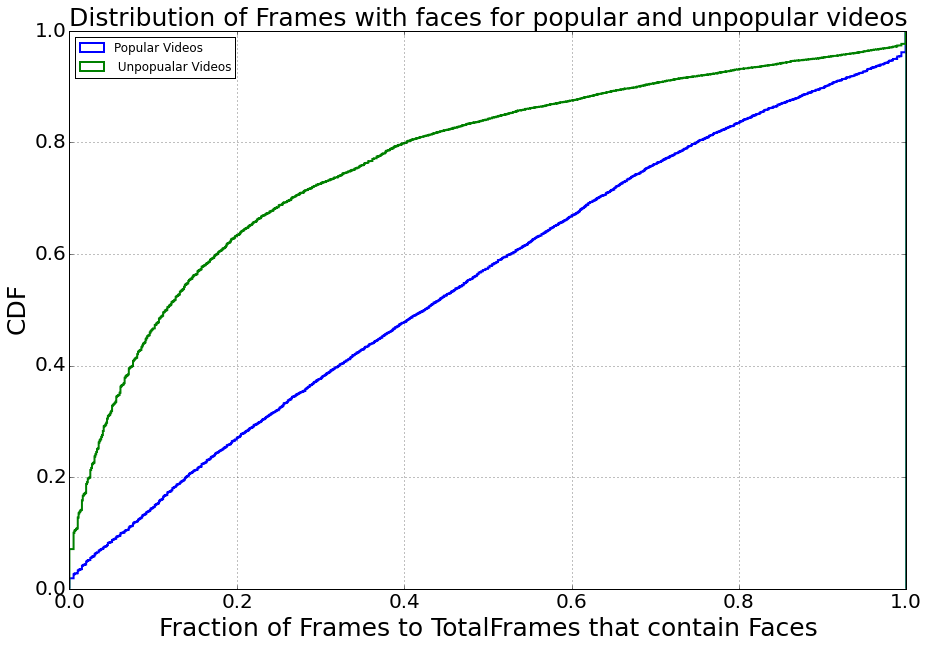
\includegraphics[width=0.45\columnwidth]{plots/FaceCDF}
%\label{fig:Face_CDF}
%}
%\caption{(a) Distribution of sentiment values for Popular and unpopular videos. The distributions follow a Gaussian like curve, but Popular videos tend to have more positive sentiments than Unpopular  (b) CDF for popular and unpopular videos. The CDF signifies the cumulative distribution of percentages of face containing frames in a vine video. The observation here is popular videos tend to have higher percentages than unpopular videos }
%\end{figure*}


%\begin{figure}[!htb]
%\centering
%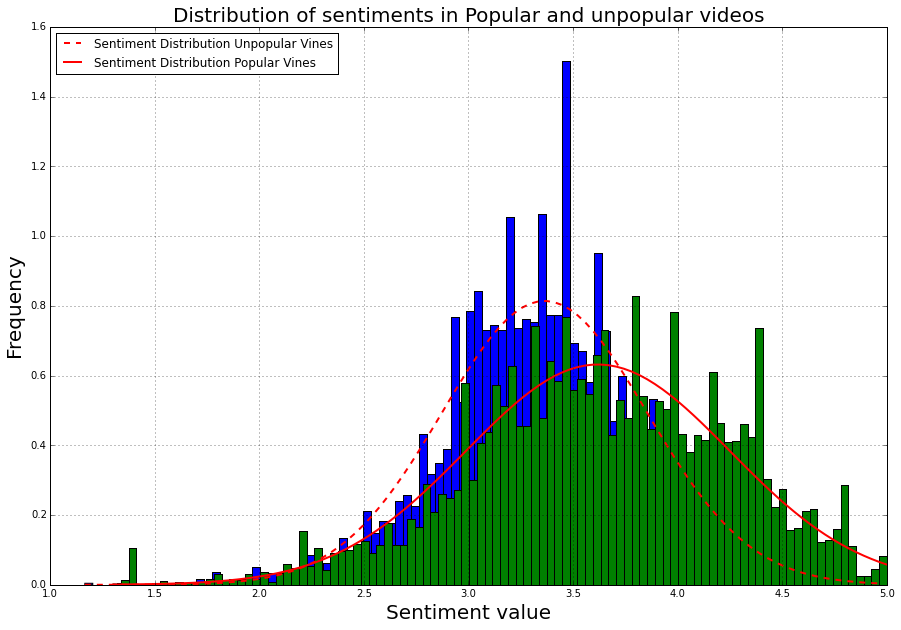
\includegraphics[width=\columnwidth]{plots/DistributionSentiments}
%\caption{\textsl{ Distribution of sentiment values for Popular and unpopular videos. The distributions follow a Gaussian like curve, but Popular videos tend to have more positive sentiments than Unpopular }}
%\label{fig:Senti_distribution}
%\end{figure}
%%



%\begin{figure}[!htb]
%\centering
%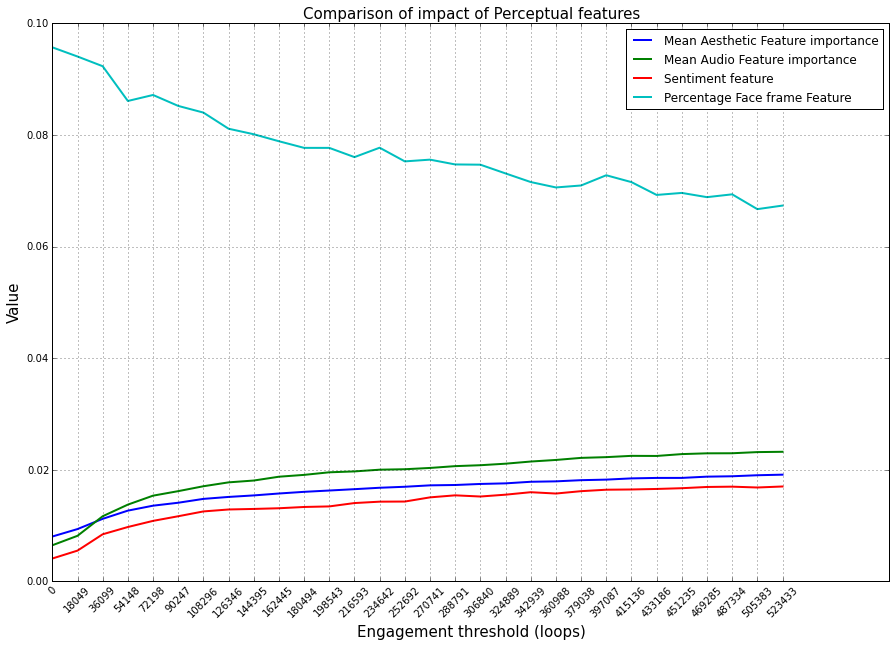
\includegraphics[width=\columnwidth]{plots/EngagementContentFeatureImpact}
%\caption{\textsl{ The plot shows change in impact of individual track features as we become more selective. The most prominent features among the content features is the presence of face. }}
%\label{fig:Feature_importance_content}
%\end{figure}


%\begin{figure}[!htb]
%\centering
%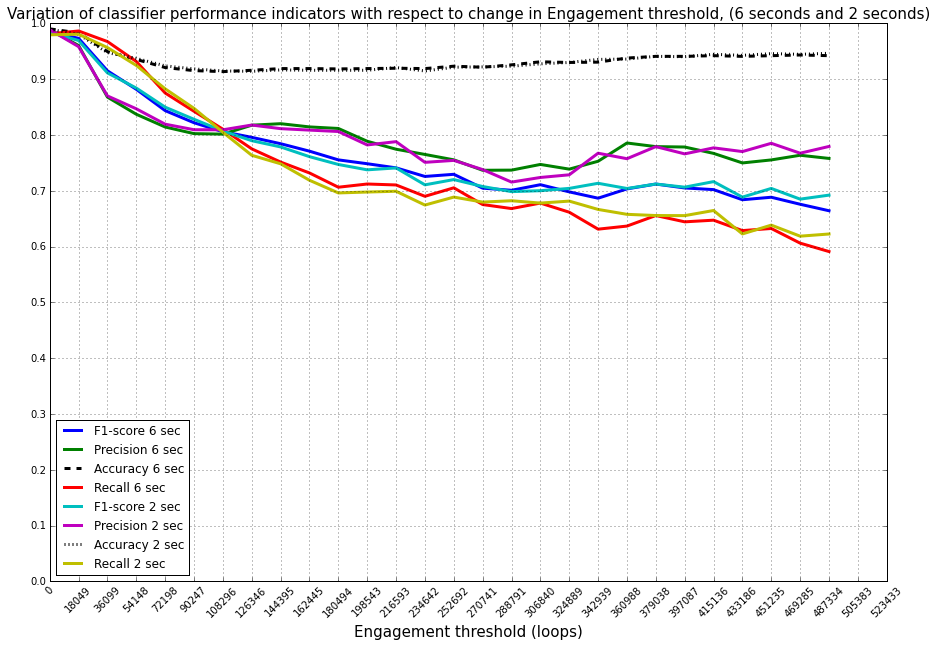
\includegraphics[width=\columnwidth]{plots/Classifier6secVs2secPerf}
%\caption{\textsl{ The plot shows comparison of the classifiers trained on the whole video features and the one trained on the first third. Both classifiers perform at par each other, and in some sense the one trained on the first third has a little better performance due to reduced noice.}}
%\label{fig:Classifier_performance}
%\end{figure}

